\chapter{Решение поставленной задачи}

\section{Анализ текста решения}

\subsection{ANTLR}
Для синтаксического анализа решения предлагается использовать генератор анализаторов для формальных языков ANTLR~\cite{antlr-site, antlr-doc}.
Чтобы получить парсер нужного языка, достаточно просто передать грамматику для данного языка в нужном формате.
ANTLR зарекомендовал себя как стабильное и удобное средство для работы с синтаксическим анализом, при этом
обладая крайне полезными для представленной работы преимуществами:
\begin{itemize}
    \item Свободное программное обеспечение.
    \item Использование единой нотации для описания лексических и синтаксических анализаторов.
    \item В репозитории разработчиков есть примеры грамматик~\cite{antlr-grammar} для многих популярных языков программирования.
    \item Множество плагинов для работы в различных средах разработки, в том числе и для Intellij IDEA, которая
        использовалась в данной работе.
    \item Возможность добавлять Java-код в грамматику с целью подстановки его напрямую в парсер. При помощи этого 
        можно запрограммировать парсер возвращать какую-либо информацию о тексте.
    \item Предоставление сообщений об ошибках и восстановление после них, в том числе корректная обработка отсутствующих узлов, 
        с последующим продолжением работы над остальным текстом. 
\end{itemize} 

Основной сложностью при работе с ANTLR стало то, что он не умеет по дереву разбора восстанавливать исходный код программы, так
как все пробелы и разделители убираются при работе лексера, и никаких обратных преобразователей не генерируется. Также проблемой
стало отсутствие возможности как-либо модифицировать построенные деревья разбора, однако обе эти проблемы решаемы.

Чтобы решить возникшие проблемы, можно модифицировать стандартную реализованную грамматику из репозитория разработчиков
добавив код, который будет строить дерево разбора, методы и структуру для которого можно реализовать отдельно на языке
Java.

После модификации грамматики работа с ANTLR сводится к нажатию пары кнопок для генерации лексера и парсера. 

\subsection{Выбор языка программирования}

Так как работать планируется со структурой кода при помощи деревьев разбора, можно не умаляя общности рассматривать один
конкретный язык программирования. Для добавления другого языка нужно будет лишь, использовав новую грамматику, получить новые лексер
и парсер, а также запрограммировать элементы структуры дерева разбора.

В данной работе будет рассматриваться язык программирования Паскаль. Это один из наиболее популярных языков для олимпиад
по программированию, который долгое время использовался для начального обучения школьников и студентов. В момент написания
работы, язык программирования сдал лидирующие позиции, однако все еще популярен и используется даже на всероссийской олимпиаде
школьников по программированию (РОИ). Язык дорабатывается по сей день в рамках языков Free Pascal~\cite{free-pascal}, 
Pascal ABC~\cite{pascal-abc} и Delphi~\cite{delphi}.

Паскаль имеет следующие особенности:
\begin{itemize}
    \item Строгая типизация.
    \item Структурное программирование.
    \item Текстовая простота.
\end{itemize}

При программировании на Паскале может сложиться ощущение, что вы программируете на английском языке, настолько синтаксис оптимизирован
для обучения.

В представленной работе будет рассмотрено избыточное подмножество изначального стандарта языка 
<<Pascal Standard>>, принятого в 1974 году.

\begin{algorithm}[!h] 
\caption{Пример программы на языке Паскаль}\label{lst1} 
\begin{lstlisting}[language=pascal]
program tmp;
const
  Author = 'Grigory';
var
  arr: array[1..2] of string;
begin
  writeln('Hi')
end.
\end{lstlisting} 
\end{algorithm}

\subsection{Дерево разбора}

Для работы с деревьями разбора по причинам, описанным ранее, необходимо было разработать собственную структуру данных, представляющую
дерево разбора, при этом позволяющую изменять свою структуру и получать код программы, которой это дерево отвечает.

Разработка данной структуры проводилась на языке программирования Java. Этот язык объектно-ориентированный, что положительно сказалось
на дизайне кода и удобстве его написания, а также ANTLR, как уже отмечалось, отлично с ним совместим.

Структура данных наследуется из основного общего класса \texttt{ASTNode}, который представляет из себя вершину дерева.
Основные типы вершин это:
\begin{itemize}
    \item переменная;
    \item константа;
    \item функция;
    \item процедура;
    \item условие;
    \item цикл с предусловием;
    \item цикл с постусловием; 
    \item цикл со счетчиком;
    \item перечисление (код между \texttt{begin} и \texttt{end});
    \item текст;
    \item тип.
\end{itemize}
Также есть вспомогательные:
\begin{itemize}
    \item двоичная операция;
    \item унарная операция;
    \item скобки;
    \item строка;
    \item универсальная.
\end{itemize}

Универсальная вершина разработана для удобства, через вершину данного типа можно разработать любую вершину, у которой есть дети.
От нее наследуются, например, вершины двоичной и унарной операций, а также вершина перечислений.  

Данная структура предназначена для представления конкретно выбранного языка, но несложно дополняется для поддержки дополнительной
функциональности языка, либо другого языка.

\begin{figure}[!h] 
\caption{Пример дерева разбора для программы из листинга~\ref{lst1}}\label{fig1} 
\begin{center}
  \makebox[\textwidth]{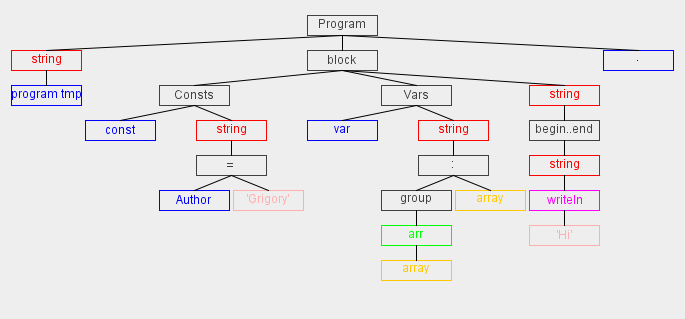
\includegraphics[width=0.9\paperwidth]{pics/tree-example.png}}
\end{center}
\end{figure}

Как было отмечено ранее, ANTLR поддерживает вставки Java-кода, поэтому стандартная грамматика была модифицирована для поддержки
разработанной структуры данных. Пример приведен в листинге~\ref{lst2}. 

\begin{algorithm}[!h] 
\caption{Пример грамматики ANTLR с вставками Java-кода}\label{lst2} 
\begin{lstlisting}[basicstyle=\small] 
constant returns [ASTNode ast]
 :unsignedNumber {
   $ast = new ConstNode($unsignedNumber.text, "num");
  }
 |sign unsignedNumber {
   $ast = new ConstNode($sign.text + $unsignedNumber.text, "sNum");
  }
 |identifier {
   $ast = new ConstNode($identifier.text, "id");
  }
 |sign identifier {
   $ast = new ConstNode($sign.text + $identifier.text, "sId");
  }
 |string {
   $ast = new ConstNode($string.text, "str");
  }
 ; 
\end{lstlisting} 
\end{algorithm}

В представленной структуре для каждого поддерева реализован метод \texttt{toString}, который сопоставляет ему
корректный код программы, который репрезентует данное поддерево. Также реализовано множество методов, которые
будут использованы по ходу продолжения работы.
%TODO перечислить?????

\section{Работа с деревьями разбора}

\subsection{Структура исправления}

Имеется два решения участника. Построим для них деревья разбора, представленные структурой данных, описанной выше, 
с помощью имеющегося парсера. 

Исследование фокусируется на <<мелких>> ошибках. Проанализируем, как выглядит поддерево дерева разбора для таких ошибок.
Утверждается, что это почти всегда лист. Действительно, если это не так, то ошибка была где-то в структуре программы,
что противоречит определению <<мелкой>> ошибки. Единственное исключение~--- это структура арифметических формул. Такие
формулы сами по себе могут сопоставляться сложным поддеревьям, но этот случай можно рассмотреть отдельно, с учетом
приоритетов, симметричности и других свойств операций. В представленной работе он не освещается.

Теперь рассмотрим структуру исправления. Исправление есть пара поддеревьев с отношением было-стало. Как было рассмотрено,
первое поддерево это всегда лист, второе же поддерево, как правило, тоже лист, но может обладать и более сложной структурой,
однако это не так важно, потому что основной задачей видеться именно найти место в новом решении, куда именно нужно попробовать 
подставить код, чем сама подстановка кода.   

Также стоит отдельно рассмотреть зависимости кода изменения от остального кода программы.
Например, когда была использована неправильная переменная, и ее заменили на другую. Однако поиск зависимостей 
осложняется по следующим причинам:
\begin{itemize}
    \item Для решения данной задачи нужен анализ решения на более высоком уровне, чем лексер-парсер, как реализовано
        в данной работе, а именно уровень семантики языка. Уровень, для реализации которого требуется написать
        подмножество компилятора, что является далеко не простой задачей.
    \item Для определения переменной, которая является такой же, что и заменяемая в другом решении, нужно знать
        все объявленные переменные, включая заголовки, подключенные библиотеки и модулю. В Паскале примерами подобной переменной,
        могут послужить \texttt{input} и \texttt{output}.
    \item Так как не всегда умеем парсить абсолютно все конструкции языка, внутри этих конструкций, тоже может что-то 
        неожиданное произойти.
\end{itemize}

Все вышеперечисленное требует того, чтобы мы умели в анализе
переменных в случае чего <<деградировать>> до поведения, в котором
неизвестно, одно и то же обозначают две переменные с одним именем, или
же нет. Которое, в общем-то, как раз и реализовано. При этом
вероятность такой деградации, в случае поддержки подмножества языка,
довольно велика.

\subsection{Поиск исправления}

Есть два дерева разбора, нужно найти в них <<отличия>>. Про искомое поддерево в первом дереве известно, что оно лист.
При этом, все остальные узлы деревьев должны быть одинаковыми по определению исправления. Случай, когда таких листьев
несколько можно свести к последовательному применению двух исправлений.

Используем алгоритм обхода графа поиском в глубину, состоянием в котором будет пара вершин: в первом и втором дереве.
\begin{itemize}
\item Рекурсивно перебирая детей вершины, спускаемся глубже.
\item Проверяем вершину первого дерева на наличие детей, если их нет, то это лист и ответом является текущее состояние.
\item Проверяем на равенство структуру вершин. Если структуры разные, то ошибка не <<мелкая>> и можно терминировать алгоритм
    с информацией об этом.
\end{itemize}

В случае, если хотим найти все мелкие ошибки, не нужно терминировать алгоритм, а просто добавлять ответы в некоторую структуру данных,
например, лист.

Также стоит отметить, что функциональность разработанной структуры данных позволяет сравнивать два узла на равенство.

\section{Применение исправления}

\subsection{Критерий <<похожести>>}
Для того, чтобы применять исправления в решении, написанном другим автором, необходимо сформулировать критерий <<похожести>>
для двух поддеревьев. В дальнейшем, именно модификация этого критерия позволит находить более сложные ошибки, чем <<мелкие>>,
вроде нерассмотренных случаев.

В данной работе, можно сказать, что два поддерева \textbf{похожи}, если:
\begin{itemize}
    \item У них одинаковая структура.
    \item Переменные одного типа, но возможно, по-разному называются.
    \item Если в поддеревьях есть константы, они могут отличаться.
\end{itemize}
Последнее полезно для типов, так как \texttt{array[1..1000] of integer} и \texttt{array[1..1001] of integer} вполне себе похожи,
но, однако, не равны.

Таким образом, возможно изменение констант и переиспользование переменных.

\subsection{Непосредственно применение}
Имеем исправления, найденные в имеющейся базе проверок решений тестирующей системы. Получаем запрос на поиск ошибки
в некотором решении, про которое известен вердикт тестирующей системы. После чего ищем все исправления в базе, 
в которых первое поддерево вырезано из решения с таким же вердиктом, как и у новоприбывшего решения. Остается, только
<<примерить>> данное исправление.

С помощью поиска в глубину найдем все похожие на первое поддерево узлы в новом решении, после чего, перебирая их по очереди,
будем подставлять вместо них второе поддерево из исправления. Простая подстановка будет корректна, так как в работе, по рассмотренным
ранее причинам, не рассматриваются зависимые от остального кода вершины. 

В случае, если первая часть изменения~--- переменная, предварительно найдем ее во второй части и при подстановке, заменим узел, на тот,
что используется в рассматриваемом решении. Данный случай, на первый взгляд, является частью зависимых случаев, однако это не совсем
правда, так как при подстановке мы не используем каких либо переменных из внешнего окружения. В прочем, если читателю
сложно представить пример такой подстановки, то он довольно прост и популярен~--- ошибка в индексе. Например, было
\texttt{a[i]}, а стало \texttt{a[i + 1]}. Довольно частая ошибка при переходе от ноль-индексации к один-индексации, либо обратно.

Возникает последний вопрос: <<что делать, если одно исправление надо применить в нескольких местах?>>.
Сложно представить, чтобы в решении задачи олимпиадного программирования было более двадцати различных мест, с одинаковой
ошибкой, поэтому предлагается, просто, попробовать подстановку в одно место, потом во все сразу, и если не поможет, то пробовать
перебирать в какие вхождения подставлять, а в какие нет. 

Подставлять во все места сразу, кажется неплохой идеей, так как немалое число исправлений часто безвредно.
Например, переход от $32$-двухбитного типа данных к $64$-битному, либо увеличение размерностей всех массивов.
То есть вероятность того, что можно исправить все, в случае, если исправить ровно одно место недостаточно, довольно велика,
однако асимптотически ничего не портит.

Также стоит отметить, что в случае синтеза исправлений автоматизация гораздо важнее времени выполнения, если оно пристойно, поэтому
подбирать какие-то более сложные схемы приоритезации попросту бессмысленно.

\chapterconclusion

\begin{enumerate}
    \item Описан способ анализа текста решения, аргументирован выбор генератора синтаксических анализаторов и языка для исследования.
    \item Описан поиск исправления по двум решениям одного учащегося, где у второго вердикт лучше чем у первого.
    \item Сформулирован критерий <<похожести>>, на основе которого разработан алгоритм применения исправления.
\end{enumerate}
